\documentclass[11pt,]{article}
\usepackage[left=1in,top=1in,right=1in,bottom=1in]{geometry}
\newcommand*{\authorfont}{\fontfamily{phv}\selectfont}
\usepackage{lmodern}


  \usepackage[T1]{fontenc}
  \usepackage[utf8]{inputenc}



\usepackage{abstract}
\renewcommand{\abstractname}{}    % clear the title
\renewcommand{\absnamepos}{empty} % originally center

\renewenvironment{abstract}
 {{%
    \setlength{\leftmargin}{0mm}
    \setlength{\rightmargin}{\leftmargin}%
  }%
  \relax}
 {\endlist}

\makeatletter
\def\@maketitle{%
  \newpage
%  \null
%  \vskip 2em%
%  \begin{center}%
  \let \footnote \thanks
    {\fontsize{18}{20}\selectfont\raggedright  \setlength{\parindent}{0pt} \@title \par}%
}
%\fi
\makeatother




\setcounter{secnumdepth}{0}

\usepackage{longtable,booktabs}

\usepackage{graphicx,grffile}
\makeatletter
\def\maxwidth{\ifdim\Gin@nat@width>\linewidth\linewidth\else\Gin@nat@width\fi}
\def\maxheight{\ifdim\Gin@nat@height>\textheight\textheight\else\Gin@nat@height\fi}
\makeatother
% Scale images if necessary, so that they will not overflow the page
% margins by default, and it is still possible to overwrite the defaults
% using explicit options in \includegraphics[width, height, ...]{}
\setkeys{Gin}{width=\maxwidth,height=\maxheight,keepaspectratio}

\title{Models and Markets: Appraising Probabilistic Predictions of the 2018 Midterm Elections  }



\author{\Large Kiernan Nicholls\vspace{0.05in} \newline\normalsize\emph{American University}  }


\date{}

\usepackage{titlesec}

\titleformat*{\section}{\normalsize\bfseries}
\titleformat*{\subsection}{\normalsize\itshape}
\titleformat*{\subsubsection}{\normalsize\itshape}
\titleformat*{\paragraph}{\normalsize\itshape}
\titleformat*{\subparagraph}{\normalsize\itshape}





\newtheorem{hypothesis}{Hypothesis}
\usepackage{setspace}

\makeatletter
\@ifpackageloaded{hyperref}{}{%
\ifxetex
  \PassOptionsToPackage{hyphens}{url}\usepackage[setpagesize=false, % page size defined by xetex
              unicode=false, % unicode breaks when used with xetex
              xetex]{hyperref}
\else
  \PassOptionsToPackage{hyphens}{url}\usepackage[unicode=true]{hyperref}
\fi
}

\@ifpackageloaded{color}{
    \PassOptionsToPackage{usenames,dvipsnames}{color}
}{%
    \usepackage[usenames,dvipsnames]{color}
}
\makeatother
\hypersetup{breaklinks=true,
            bookmarks=true,
            pdfauthor={Kiernan Nicholls (American University)},
             pdfkeywords = {Prediction markets, election forecasting, FiveThirtyEight, PredictIt},  
            pdftitle={Models and Markets: Appraising Probabilistic Predictions of the 2018 Midterm Elections},
            colorlinks=true,
            citecolor=blue,
            urlcolor=blue,
            linkcolor=magenta,
            pdfborder={0 0 0}}
\urlstyle{same}  % don't use monospace font for urls

% set default figure placement to htbp
\makeatletter
\def\fps@figure{htbp}
\makeatother



% add tightlist ----------
\providecommand{\tightlist}{%
\setlength{\itemsep}{0pt}\setlength{\parskip}{0pt}}

\begin{document}
	
% \pagenumbering{arabic}% resets `page` counter to 1 
%
% \maketitle

{% \usefont{T1}{pnc}{m}{n}
\setlength{\parindent}{0pt}
\thispagestyle{plain}
{\fontsize{18}{20}\selectfont\raggedright 
\maketitle  % title \par  

}

{
   \vskip 13.5pt\relax \normalsize\fontsize{11}{12} 
\textbf{\authorfont Kiernan Nicholls} \hskip 15pt \emph{\small American University}   

}

}








\begin{abstract}

    \hbox{\vrule height .2pt width 39.14pc}

    \vskip 8.5pt % \small 

\noindent Forecasting models and prediction markets are two methods of generating
probabilistic predictions of upcoming elections. The efficient market
hypothesis holds that fair markets should incorporate all information,
including public models, in price discovery. This paper compares the
market price on the \emph{PredictIt} exchange to the model probability
released by the data journalist at \emph{FiveThirtyEight}. Sample
includes the last 90 days of 115 races in the 2018 midterm elections. In
a test for equal proportion of accurate predictions, the markets
outperformed the model to a statistically significant degree (market:
86.03\%, model: 83.81\%, p = 0.00004166). In a more comprehensive test
of forecast skill, there was no statistical difference in Brier scores
(market: 0.1084, model: 0.1091, p = 0.7346).


\vskip 8.5pt \noindent \emph{Keywords}: Prediction markets, election forecasting, FiveThirtyEight, PredictIt \par

    \hbox{\vrule height .2pt width 39.14pc}



\end{abstract}


\vskip 6.5pt

{
\hypersetup{linkcolor=black}
\setcounter{tocdepth}{2}
\tableofcontents
}

\noindent \doublespacing \hypertarget{introduction}{%
\section{Introduction}\label{introduction}}

In the wake of the 2016 Presidential election, pundits and voters alike
were stunned by the seemingly impossible outcome. Dozens of respected
prognosticators issued predictions that were, in hindsight, comically
overconfident. Comedians, Presidents, and journalists alike seemed all
but certain in a Clinton victory. Even the most quantitative efforts
fell short. After the 2012 Presidential election, it seemed like ``big
data'' was the solution to prediction. Nate Silver's fledgling site
\emph{FiveThirtyEight} made news by using a polling aggregation model to
accurately predict the popular vote winner in all 51 states. In 2016,
such efforts proved inaccurate. The most egregious errors came from the
likes of the Princeton Election Consortium and Huffington Post, who each
gave Trump less than a 2\% probability of victory. The least bullish of
these incorrect odds was \emph{FiveThirtyEight's}, at a 29\% for Trump.
This number was so high that it provoked criticism from the Huffington
Post's Ryan Grim:

\begin{quote}
I get why Silver wants to hedge. It's not easy to sit here and tell you
that Clinton has a 98 percent chance of winning. Everything inside us
screams out that life is too full of uncertainty, that being so sure is
just a fantasy. But that's what the numbers say. What is the point of
all the data entry, all the math, all the modeling, if when the moment
of truth comes we throw our hands up and say, hey, anything can happen.
If that's how we feel, let's scrap the entire political forecasting
industry. (Grim 2016)
\end{quote}

This quotation is particularly thought provoking. Both Silver and Grim
built election forecasting models using the same general set of inputs,
but used those numbers to tell a different story about how the election
was going to unfold. These models have a responsibility to accurately
convey information and may very well influence the very event they are
trying to predict. If these quantitative forecasting models could be
wrong in 2016 (to various degrees), should we consider looking for
alternative methods? There has been some focus in recent years on the
prediction market (also known as information or decision markets) as one
such tool to generate similarly probabilistic forecasts. Might these
markets have a role to play in prediction elections? Can they outperform
the forecasting model that has become such a widely used tool in recent
years, and If so, under what conditions? To answer these questions, I
will be comparing the market prices from the \emph{PredictIt} exchange
against the \emph{FiveThirtyEight} model for the 2018 midterm elections.

\hypertarget{literature}{%
\section{Literature}\label{literature}}

Prediction markets are a relatively new but fairly researched tool for
assessing the likelihood of events. There are a numerous academic
investigations into the quality of these predictions across a number of
field. These studies have become more popular in the 21st century, as
the advent of the internet makes the operation of large scale market
exchanges significantly easier. As far as political predictions go, the
vast majority of these studies compare prediction markets to opinion
polling (simply aggregated at the most) for Presidential races. There is
room in the literature to study the ability of prediction markets in
congressional races against the more comparable probabilistic
forecasting models.

\hypertarget{theory}{%
\subsection{Theory}\label{theory}}

Kenneth Oliven and Thomas Rietz explored the economic forces of
prediction markets in their paper \emph{Suckers Are Born but Markets Are
Made: Individual Rationality, Arbitrage, and Market Efficiency on an
Electronic Futures Market} (2004). The paper looked at the individual
economic incentives of traders betting on the 2004 presidential election
on the Iowa Election Market. The paper specifically explores the way
prediction markets fall short of the perfect efficiency claimed by the
efficient market hypothesis. The theory is primarily based around two
theories of rational traders: (1) the law of one price (LOOP) and (2)
arbitrage-free pricing. Since the exchanges hold a single market related
to a given election, the price of that election should be the sole
reflection of available information. The authors argue that the IEM and
other prediction markets are an ideal setting to explore whether or not
traders conform to these theories.

Traders on these markets are theoretically more informed than the
population at large, but the paper finds that prediction markets are
often populated by mistake-prone and biased traders ``prone to
behavioral anomalies predicted by behavioral finance'' (336). The
inefficiency from these errors are what make markets useful for
individual traders. In a perfectly efficient market, it's impossible to
``beat'' the market price which should already encompass all
information. The authors conclude that ``{[}a{]} fundamental property of
markets is that marginal, not average, traders determine prices. Who
marginal traders are and how they set prices determine whether markets
are efficient.'' (337). The traders who take the prices set by marginal
traders are more mistake prone and less rational. On the IEM, the study
found that not all traders need to be rational for the market to
``generate efficient prices in spite of bias'' (337).

\hypertarget{uncertainty}{%
\subsection{Uncertainty}\label{uncertainty}}

Prediction markets and forecasting models are two predictive methods
suited for comparison because both aim to produce a similarly
probabilistic prediction. That is, both methods generate a prediction
that expresses the given probability of an event occurring that allows
observers to evaluate uncertainty in a quantifiable way. This value of
uncertainty evaluation was explored by Ray Fair in his paper
\emph{Interpreting the Predictive Uncertainty of Elections} (2009). Fair
distinguishes between the kind of event uncertainty expressed by
prediction markets and forecasting models and the sample-size
uncertainty expressed by the margin of error around an opinion poll
average. Fair presents a theory of uncertainty that ``there are a number
of possible `conditions' of nature that can exist on election day, of
which one is drawn. The uncertainty is which condition will be drawn''
(612).

Fair has us imagine \(n\) possible conditions of nature, where \(1/n\)
is the probability of each condition occurring. If in \(p\) percent of
the n conditions a given candidate wins the election, then \(p\) is the
probability that said candidate will win on election day. Over the
course of the election, every action affects the possible set of
conditions that might occur. The challenge of uncertainty is determining
what the probabilities are without knowing all possible conditions. The
author identifies prediction markets as one tool to estimate that
uncertainty by crowd-sourcing and aggregation of many estimated
conditions and their likelihood. Forecasting models perform the same
function by simulating many potential conditions and calculating p
manually.

Uncertainty is more frequently expressed using the standard error of a
opinion poll. Fair contrasts these two fundamentally different types of
uncertainty estimates by imagining an opinion poll being held the day
before the election that polled every single eligible voter. The same
size of this poll is so large that the standard error would be zero, but
real uncertainty still exists. Voters change their mind, circumstances
dictates who can make it to the polls, even weather affects the mood of
voters and causes real uncertainty. Even if such a poll existed, the
forecasting model and prediction market would likely produce
probabilistic estimates less than 100\% for the winner predicted by the
poll. This difference in types of uncertainty means market predictions
are best compared to a similarly probabilistic prediction, like those
generated by the newest iterations of the forecasting model.

\hypertarget{legality}{%
\subsection{Legality}\label{legality}}

One of the most important things to note about prediction markets is the
questionable legality of their use. While gambling in general is not
illegal under federal law, online gambling has been generally prohibited
under the Unlawful Internet Gambling Enforcement Act of 2006.
Additionally, political gambling in particular is even further
regulated. In a paper titled \emph{The Promise of Prediction Markets},
22 researchers, including the likes of Kenneth Arrow and Philip Tetlock,
encourage the United States government to relax regulation on prediction
markets (2008). The paper begins by citing growing evidence that such
markets offer ``lower prediction error than conventional forecasting
methods.'' The authors further explain that markets can be used to
improve decision making in a number of fields, and that regulation is
preventing these tools from being used to their full potential. While
the Internet makes it easy enough to skirt such regulation by using
prediction markets hosted offshore, the authors contend such lengths are
prohibitive to their use by the general public.

The authors conclude by proposing a set of regulatory reforms intended
to safely promote the use of prediction markets so that the industry may
better gauge their full capabilities. In the regards to specifically
political gambling, one such proposal is the ``no-action letter'' issued
by the Commodity Futures Trading Commission (CFTC) for institutions
which strictly violate law but will not be prosecuted. At the time of
writing, only the Iowa Election Market (IEM) at the The University of
Iowa had received such a letter. As of 2019, both the IEM and the
Victoria University of Wellington, New Zealand's PredictIt exchange,
operate under such letters of no-action. The authors urge the CTFC to
establish more permanent and relaxed guidance so that markets can
operate more freely without fear of unanticipated prosecution. This
paper further urges Congress to support the study of prediction markets
by giving the CFTC the necessary funding to regulate a growing industry.
The legal status of prediction markets must be kept in mind when
discussing their feasibility as an alternative tool to the unambiguously
legal forecasting model. Furthermore, the necessary regulatory
compromises do inhibit the free market forces theoretically needed for
proper price discovery and prediction.

\hypertarget{manipulation}{%
\subsection{Manipulation}\label{manipulation}}

One reason such reason regulation is ultimately necessary is the
potential for market manipulation. This possibility is discussed by Iowa
University researchers Joyce Berg and Thomas Rietz in their paper
\emph{Market Design, Manipulation, and Accuracy in Political Prediction
Markets} (2014). The paper analyzes two markets set up to predict the
2012 presidential election; the first has traders bet on the division of
the popular vote, where the second predicted the overall winner of the
popular vote. The authors note that the IEM vote-share prediction was
closer to the actual election number than 74\% of individual opinion
polls. The paper discusses the possibility that deliberate manipulate
might affect this accuracy and conclude with two market techniques to
discourage manipulation. The paper uses the Securities and Exchange Act
definition of price manipulation: ``To effect, alone or with 1 or more
other persons, a series of transactions\ldots{} raising or depressing
the price of (a) security, for the purpose of inducing the purchase or
sale of such security by others.''

Under the typical conditions, the intentions of the voters drive the
actions of traders; that is, traders on the market look to place bets in
line with their prediction of voter behavior. The authors explain that
``The causal logic underlying prediction market manipulation goes the
opposite direction: market prices drive voter actions, affecting them in
predictable ways'' (293). The authors evaluate the possibility that
malicious traders might directly manipulate the price to affect voter
behavior and profit off the outcome they directly influenced. The paper
cites previous research which shows such manipulate is unlikely in the
long term (Rhode and Strumpf 2006). Account limits and linked unit
portfolios are two features intended to mitigate the potential for
manipulation. Together, these two features require ``{[}a{]} manipulator
who alters bid/ask queues must maintain these bids and asks against the
profit motives of hundreds of other traders with hundreds of thousands
of dollars'' (296). They found little evidence that the IEM can be
manipulated in the long run. This is good evidence to support the use of
prediction markets as a tool in election forecasting.

\hypertarget{methodology}{%
\section{Methodology}\label{methodology}}

To compared prediction markets against forecasting models, I will be
using the historical probabilistic data from each. I theorize that the
prediction markets will outperform the forecasting market early in the
election cycle, when polling is sparse and the model must rely on less
quantitative data with a greater degree of uncertainty. To test this
theory, I will be assessing the daily prediction from both methods
against the eventually winner of that race and calculating the
proportion of correct predictions for each model. To understand how
these two predictive methods might compare to one another, we first have
to understand the basic conception of how each model produces
probabilistic predictions; this similarity is key to comparing these two
methods, as opposed to the vote share division of opinion polls or the
typically binary prediction of pundits. Understanding the process behind
each predictive method is key to understanding their comparative value
and roles in predicting elections.

\hypertarget{predictive-tools}{%
\subsection{Predictive Tools}\label{predictive-tools}}

Forecasting models are the natural evolution of opinion polling, the
most basic form of election forecasting. Opinion polls as a predictive
method date back hundreds of years and rely on equal probability
sampling of a population to draw an unbiased sample that can be used to
more easily determine the voting intentions of the overall population.
These polls fail to perfectly predict the election due to both sampling
and statistical errors. To overcome these shortcomings, prognosticators
have taken to aggregating many polls and averaging them together. The
Law of Large Numbers holds that the mean of repeated samples (polls) of
the same population result in a new mean closer to the truth.
Forecasting models take poll aggregation and various other quantitative
inputs and simulate the election to produce a \emph{probabilistic} view
of potential outcomes (i.e., ``70\% chance of winning'' rather than
``56\% of the vote'').

I will be using the \emph{FiveThirtyEight} forecasting model, as they
have a proven record of accuracy and make their output data free to the
public. The exact code of the \emph{FiveThirtyEight} model is
proprietary, but we have a general idea of what data is used with what
weight. From the public information we have, the model incorporates: (1)
aggregate polls weighted for past accuracy and other effects, (2) an
algorithm to impute polling for districts without any, and (3)
historically useful ``fundamental'' factors: incumbency, fundraising,
scandals, the generic ballot, past election margin, and challenger's
experience, etc. These inputs are used to generate a likely division of
the vote in that race. Next, the model makes the important additional of
incorporating uncertainty. This addition of uncertainty separates the
model from other simpler poll aggregators and allows us to consider
their results side by side with prediction markets.

Uncertainty is estimated by evaluating a number of historically useful
indicators in the creation of a probability distribution.
\emph{FiveThirtyEight} has found that uncertainty is greater when: the
election is further away in time, there are more undecided or
third-party voters, there are fewer overall polls, those polls show a
more lopsided race, the polls disagree with one another, and those polls
disagree with the fundamental variables of the state. For each race
being predicted, these factors are considered and a probability
distribution is generated around the estimated division of the vote. The
model relies on a Monte Carlo simulation to turn this distribution into
an expression of probability. The model randomly draws a share of votes
from the distribution (i.e., simulates an election). The percentage of
drawn divisions with one candidate winning is analogous to that
candidates probability of winning on election day. This process allows
forecasting models to incorporate a range of historically useful data in
the generation of probabilistic predictions.

Prediction markets, on the other hand, generate similar predictions by
having self-interested and risk-averse traders buy and sell futures
contracts tied to the predefined set of outcomes to an event. Instead of
relying on equal probability sampling of a population to draw an
unbiased sample and determine a prediction, prediction markets rely on
the self-interest of biased yet risk averse traders. Despite the
political bias of each individual trader, market theory dictates that
each should be willing to place bets that aim to net profit, regardless
of political outcome. On these markets, traders buy and sell futures
contracts tied to a specific event or point in the future. When a trader
``buys'' a share of a given market, they are really entering into a
contract with another trader on the other side to pay the full price of
the contract to the holder of the correct contract. The goal is to make
a profit by buying shares of events you think are likely for the lowest
possible price. To buy these shares, another trader needs to believe
that the inverse of your prediction is true.

For example, if I believe the Democrat is a strong favorite the win the
election in a given district, I would be willing to buy shares tied to
that outcome for any price less than my prior understanding. The
efficient market hypothesis holds market prices reflect all available
information. As a trader, I should consider public opinion polls,
insider information, my expert analysis, or maybe just a gut feeling in
my assessment of the election. If from all this information I determine
that probability of the Democratic candidate winning to be 75\%, it's in
my self interest to buy contracts for any price below \$0.75. Like any
market, the price of the contracts are determined by supply and demand.
Prediction markets determine the probability of events the same way the
stock market predicts the future earnings of a company by supply and
demand of the securities. If I'm right and the Democrat does win, each
of the shares executes for \$1.00 and I get my \$0.75 back, plus the
\$0.25 from every wrong contract (minus an exchange fee). If more
traders believe the probability is above the market price, they will
look to buy those shares, increasing demand and the equilibrium price.
This is the general process by which prediction markets aggregate many
individual beliefs into a single agreed upon probability.

Since these two predictive tools both produce similar probabilistic
predictions through different means, they can be compared side by side.
Before comparing the data from each method, we must acknowledge the
recursive relationship between them. It is the nature of prediction
markets to contain auto-correlated feedback loops. The two methods do
not produce their respective predictions independent of one another;
traders can and do use the public forecasting model in their analysis.
There is quite possibly a negligible relationship in the opposite
direction, with voters finding the relatively unknown prediction markets
and changing their assumptions accordingly, which would affect the
polling and forecasting model. This relationship does not disqualify
this study. We might rephrase the research question, instead asking if
prediction markets improve or dilute the forecasting model prediction
with additional crowd-sourced information. There is still value in
exploring each method's ability to predict future events from an
overlapping source of inputs.

\hypertarget{predictive-data}{%
\subsection{Predictive Data}\label{predictive-data}}

Now that we understand the source of each set of predictions, I will
briefly describe the nature of the data that will be used to asses their
respective predictive capabilities. All data used in this paper is
freely available for academic research. An archive of all public
information has been created on the free Internet Archive. Additionally,
the source code for this paper and all analysis is hosted on a public
GitHub repository, which can be cloned to reproduce findings exactly.
All software needed to produce the same results is free and open source.

All data sets is collected, formatted, combined, and analyzed using the
statistical computing language R (R Core Team 2018) and a handful of
specialized packages: \texttt{readr} (Wickham, Hester, and Francois
2018) and \texttt{wayback} (Rudis 2017) for data collection;
\texttt{dplyr} (Wickham et al. 2019) and \texttt{tidyr} (Wickham and
Henry 2019) for data manipulation; \texttt{stringr} (Wickham 2019) and
\texttt{lubridate} (Grolemund and Wickham 2011) for character and date
strings; \texttt{ggplot2} (Wickham 2016) for visualization; and
\texttt{verification} (Research Applications Laboratory 2015) for
forecast analysis. See the appendix for all the R code used in this
project, which can be run sequentially to reproduce my findings.

\hypertarget{markets-data}{%
\subsection{Markets Data}\label{markets-data}}

Prediction market data comes courtesy of the PredictIt exchange, which
is run by the University of New Zealand at Wellington with logistical
support from Aristotle Inc.~PredictIt provides historical market data to
partnered academic researchers free of charge as part of their ``no
action'' agreement with the Commodity Futures Trading Commission.
PredictIt hosts markets for midterm races of interest. Each race is
comprised of contracts tied to the outcome, either
``Democrat/Republican'' or ``Yes/No'' depending on whether the market
question is phrased around a generic congressional election or the
reelection of an incumbent. The public PredictIt API was scraped before
the election to extract all market IDs related to the midterm elections.
Those IDs were passed to the PredictIt contact, who returned a single
file containing the price history of all markets. The market data set
contains 45,037 rows with 11 variables (Table 1). Each row represents a
single day's contract price history (opening, closing, low, and high
price). The data spans from January 27th, 2017 to December 3rd, 2018. I
will be operationalizing the closing contract price as that day's
``final'' prediction as to the candidate's probability of victory.

\begin{longtable}[]{@{}lllrr@{}}
\caption{Market Data Sample (Random)}\tabularnewline
\toprule
Date & Market & Contract & Volume & Price\tabularnewline
\midrule
\endfirsthead
\toprule
Date & Market & Contract & Volume & Price\tabularnewline
\midrule
\endhead
2017-05-24 & CRUZ.TXSENATE.2018 & NA & 581 & 0.75\tabularnewline
2017-10-29 & HURD.TX23.2018 & NA & 0 & 0.41\tabularnewline
2018-04-10 & WA08.2018 & DEM.WA08.2018 & 20 & 0.72\tabularnewline
2018-04-26 & PA09.2018 & DEM.PA09.2018 & 0 & 0.20\tabularnewline
2018-06-14 & MI11.2018 & GOP.MI11.2018 & 0 & 0.42\tabularnewline
2018-07-30 & CASE.PASENATE.2018 & NA & 0 & 0.93\tabularnewline
2018-08-26 & FISC.NESENATE.2018 & NA & 30 & 0.93\tabularnewline
2018-09-14 & AZ02.2018 & GOP.AZ02.2018 & 1 & 0.17\tabularnewline
2018-10-29 & BACO.NE02.2018 & NA & 979 & 0.80\tabularnewline
2018-11-04 & CURB.FL26.2018 & NA & 107 & 0.47\tabularnewline
\bottomrule
\end{longtable}

\hypertarget{model-data}{%
\subsection{Model Data}\label{model-data}}

Forecasting model data come courtesy of the data journalists at
\emph{FiveThirtyEight}, who were closest to reality in 2016, have a
track record of success, and is one of the few forecasts to continue
their work into the midterm elections. Again, \emph{FiveThirtyEight's}
exact model is proprietary, but they provide the top-level output to the
public. The data comes in two separate files, one for the 435 House
races and another for the 35 Senate elections that year. Combined, the
two data sets contain 328,113 rows of 13 variables (Table 2). Each row
represents a single day's predicted probability of a given candidate's
victory. The data set contains daily predictions from August 1st to
election day on November 8th of 2018.

\begin{longtable}[]{@{}llrllrr@{}}
\caption{House Model Data Sample (Head)}\tabularnewline
\toprule
Date & State & District & Party & Incumbent & Mean Share &
Probability\tabularnewline
\midrule
\endfirsthead
\toprule
Date & State & District & Party & Incumbent & Mean Share &
Probability\tabularnewline
\midrule
\endhead
2018-08-01 & AK & 1 & R & TRUE & 49.35 & 0.718\tabularnewline
2018-08-01 & AK & 1 & D & FALSE & 44.11 & 0.282\tabularnewline
2018-08-01 & AK & 1 & NA & FALSE & 6.54 & 0.000\tabularnewline
2018-08-01 & AL & 1 & R & TRUE & 64.90 & 0.999\tabularnewline
2018-08-01 & AL & 1 & D & FALSE & 35.10 & 0.001\tabularnewline
2018-08-01 & AL & 2 & R & TRUE & 58.23 & 0.973\tabularnewline
2018-08-01 & AL & 2 & D & FALSE & 41.77 & 0.027\tabularnewline
2018-08-01 & AL & 3 & R & TRUE & 62.27 & 0.997\tabularnewline
2018-08-01 & AL & 3 & D & FALSE & 37.73 & 0.003\tabularnewline
2018-08-01 & AL & 4 & R & TRUE & 76.32 & 1.000\tabularnewline
\bottomrule
\end{longtable}

\hypertarget{combined-data}{%
\subsection{Combined Data}\label{combined-data}}

Each data set is combined by creating a common \texttt{race} key
variable so that observations from the same day for the same race can be
compared. With this key variable, a relational join is performed to put
the prediction variables side by side. It's important to note that only
predictions contained in both data sets are kept; while the model
predicts all 470 races every day, betting markets only exists for races
of interest. This means the races predicted by both data sets are
significantly more uniformly distributed (Figure 1). This new
distribution is a sample of total races, one with a much greater
proportion of toss-up elections. It's a fair assumption to say

\begin{figure}
\centering
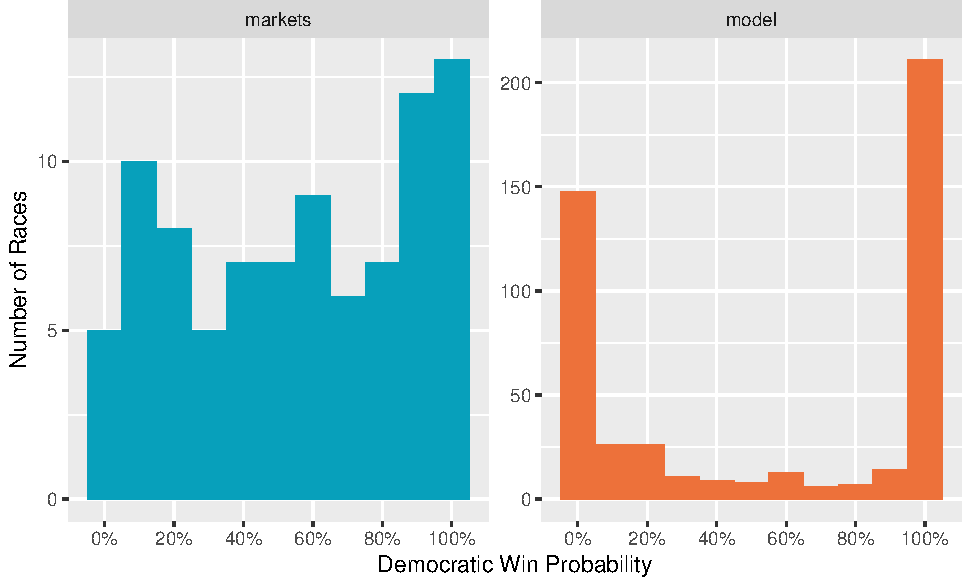
\includegraphics{paper_files/figure-latex/plot_dist-1.pdf}
\caption{Proportion of Correct Predictions by Week}
\end{figure}

The data is then filtered to remove redundant predictions by keeping
only Democratic predictions (or the inverse of Republican predictions).
Finally, the data is converted in a ``long'' rather than ``wide''
format, with each row representing a unique prediction and a new
variable indicating the method used to generate it. In this ``tidy''
format, the two groups can be easily visualized and compared against one
another. Figure 2 depicts the difference in predictions in the sample.
If the two methods were exactly the same, all races would fall on on the
\(x = y\) line. For races plotted in quadrant 1, the Democratic
candidate is predicted to win by the market and predicted to lose by the
mode. The inverse is true for quadrant 4. In quadrants 2 and 3, both
methods are in agreement in their predictions.

\begin{figure}
\centering
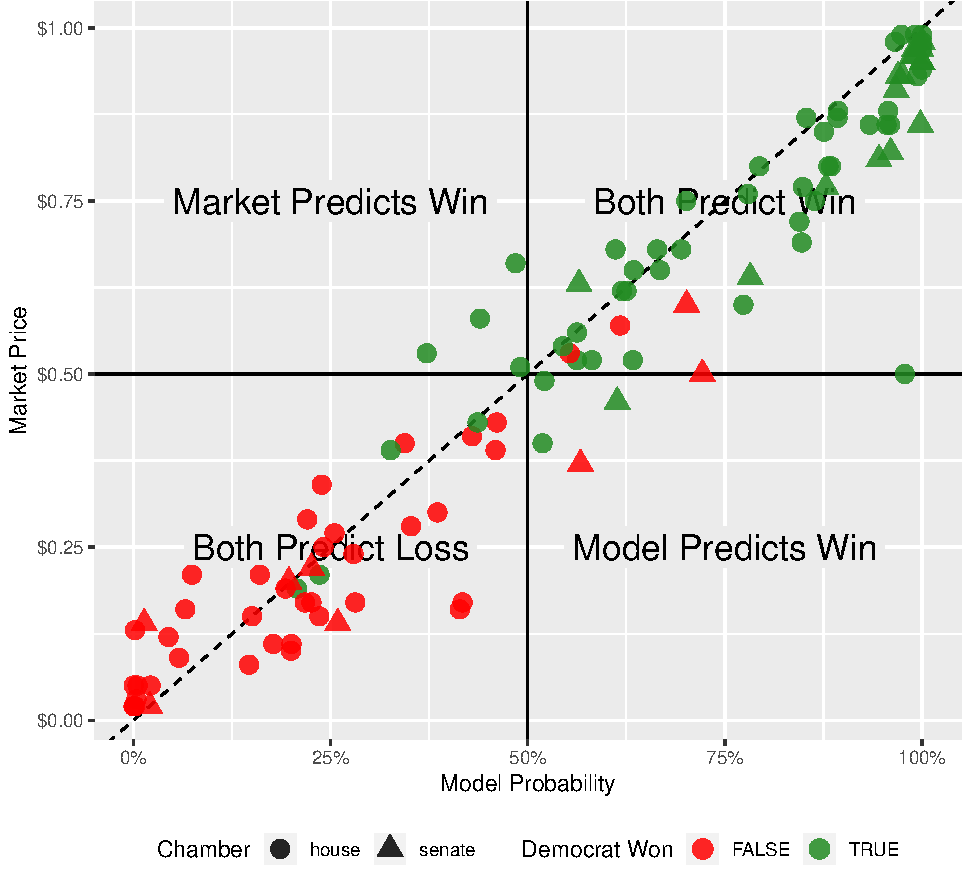
\includegraphics{paper_files/figure-latex/plot_cart-1.pdf}
\caption{Probability Comparisons (Nov.~5)}
\end{figure}

\hypertarget{results}{%
\section{Results}\label{results}}

When assessing predictions, the most obvious metric is whether they are
simply right or wrong. In the combined data set, there are 17,500
predictions and each of them ultimately makes a binary prediction on
whether a candidate will win or lose that election. If we want to
evaluate two methods of prediction, it makes sense to simply check which
method was able to accurately predict more elections. The initial null
hypothesis for this study held that there would be no difference in the
overall proportion of accurate predictions over the course of the
election. The alternative hypothesis being that there is in fact some
difference, proving one method to be superior in prediction
Congressional races. I chose to test the entire length of the campaign,
as opposed to the ``final'' election night prediction, to evaluate each
method as a daily predictive tool. Election prediction serves more roles
than simply getting it right on election night; campaign operatives,
party leaders, and data journalists rely on daily quantitative
predictions to rigorously interpret changes in the campaign.

\hypertarget{proportion}{%
\subsection{Proportion}\label{proportion}}

To run a two-sample hypothesis test of equal proportion, the combined
prediction data would have to be compared with eventual election
results. Those results were provided by the team at
\emph{FiveThirtyEight} and the \emph{ABC News} decision desk. By
formatting the results in the same was as prediction data, a third
simple relational join can be performed. This result is compared to the
binary win/loss prediction and a new logical value is created to
represent the prediction's ultimate accuracy (Table 4). The proportion
of ``hit'' predictions for each method is compared. From this test, we
can confidently reject our null hypothesis and accept the alternative
hypothesis. With a chi squared value of 16.8 and a p-value of 0.0000417,
we are confident the proportion of correct predictions is not equal to
zero. In our sample, 86.03\% of predictions made by traders on the
PredictIt exchanged proved correct. With a 95\% confidence, we know
proportion value is 1.16 to 3.3\% greater than the 83.81\% of correct
predictions made by the \emph{FiveThirtyEight} model (Table 5).

\begin{longtable}[]{@{}lllrlll@{}}
\caption{Tidy Comparison Data}\tabularnewline
\toprule
Date & Race & Method & Probability & Prediction & Election &
Accurate\tabularnewline
\midrule
\endfirsthead
\toprule
Date & Race & Method & Probability & Prediction & Election &
Accurate\tabularnewline
\midrule
\endhead
2018-08-01 & AZ-S1 & market & 0.660 & TRUE & TRUE & TRUE\tabularnewline
2018-08-01 & AZ-S1 & model & 0.738 & TRUE & TRUE & TRUE\tabularnewline
2018-08-01 & CA-12 & market & 0.910 & TRUE & TRUE & TRUE\tabularnewline
2018-08-01 & CA-12 & model & 1.000 & TRUE & TRUE & TRUE\tabularnewline
2018-08-01 & CA-22 & market & 0.300 & FALSE & FALSE &
TRUE\tabularnewline
2018-08-01 & CA-22 & model & 0.049 & FALSE & FALSE & TRUE\tabularnewline
2018-08-01 & CA-25 & market & 0.610 & TRUE & TRUE & TRUE\tabularnewline
2018-08-01 & CA-25 & model & 0.745 & TRUE & TRUE & TRUE\tabularnewline
2018-08-01 & CA-39 & market & 0.610 & TRUE & TRUE & TRUE\tabularnewline
2018-08-01 & CA-39 & model & 0.377 & FALSE & TRUE & FALSE\tabularnewline
\bottomrule
\end{longtable}

\begin{longtable}[]{@{}cccccc@{}}
\caption{2-sample test for equality of proportions with continuity
correction: \texttt{Markets\ vs\ Model}}\tabularnewline
\toprule
\begin{minipage}[b]{0.17\columnwidth}\centering
Test statistic\strut
\end{minipage} & \begin{minipage}[b]{0.05\columnwidth}\centering
df\strut
\end{minipage} & \begin{minipage}[b]{0.18\columnwidth}\centering
P value\strut
\end{minipage} & \begin{minipage}[b]{0.24\columnwidth}\centering
Alternative hypothesis\strut
\end{minipage} & \begin{minipage}[b]{0.10\columnwidth}\centering
Markets\strut
\end{minipage} & \begin{minipage}[b]{0.10\columnwidth}\centering
Model\strut
\end{minipage}\tabularnewline
\midrule
\endfirsthead
\toprule
\begin{minipage}[b]{0.17\columnwidth}\centering
Test statistic\strut
\end{minipage} & \begin{minipage}[b]{0.05\columnwidth}\centering
df\strut
\end{minipage} & \begin{minipage}[b]{0.18\columnwidth}\centering
P value\strut
\end{minipage} & \begin{minipage}[b]{0.24\columnwidth}\centering
Alternative hypothesis\strut
\end{minipage} & \begin{minipage}[b]{0.10\columnwidth}\centering
Markets\strut
\end{minipage} & \begin{minipage}[b]{0.10\columnwidth}\centering
Model\strut
\end{minipage}\tabularnewline
\midrule
\endhead
\begin{minipage}[t]{0.17\columnwidth}\centering
16.79\strut
\end{minipage} & \begin{minipage}[t]{0.05\columnwidth}\centering
1\strut
\end{minipage} & \begin{minipage}[t]{0.18\columnwidth}\centering
4.166e-05 * * *\strut
\end{minipage} & \begin{minipage}[t]{0.24\columnwidth}\centering
two.sided\strut
\end{minipage} & \begin{minipage}[t]{0.10\columnwidth}\centering
0.8603\strut
\end{minipage} & \begin{minipage}[t]{0.10\columnwidth}\centering
0.8381\strut
\end{minipage}\tabularnewline
\bottomrule
\end{longtable}

We can further explore these proportions over time to explore the
difference in accuracy over time. Such an analysis confirms my
hypothesis that the predictions markets would outperform the
polling-reliant model earlier in the election cycle. In the early weeks
of the campaign, the prediction markets were producing prices that
accurately reflected over 90\% of races eventually winner. Compare this
to the roughly 85\% accuracy from the forecasting model. It's worth
noting that the number of predictions made each day is not consistent.
Over the course of the campaign, markets for more and more races were
added to the exchange, from 121 on August 1st to 183 on November 5th
(Figure 4). Over this period, the mean of all market prices for
Democrats decreased from \$0.60 to \$0.52. This might indicate that the
additional markets added over the course of the election might have a
Republican bias. Although it's very possible that the overall trend of
the election was shifting towards the Republican party.

\begin{figure}
\centering
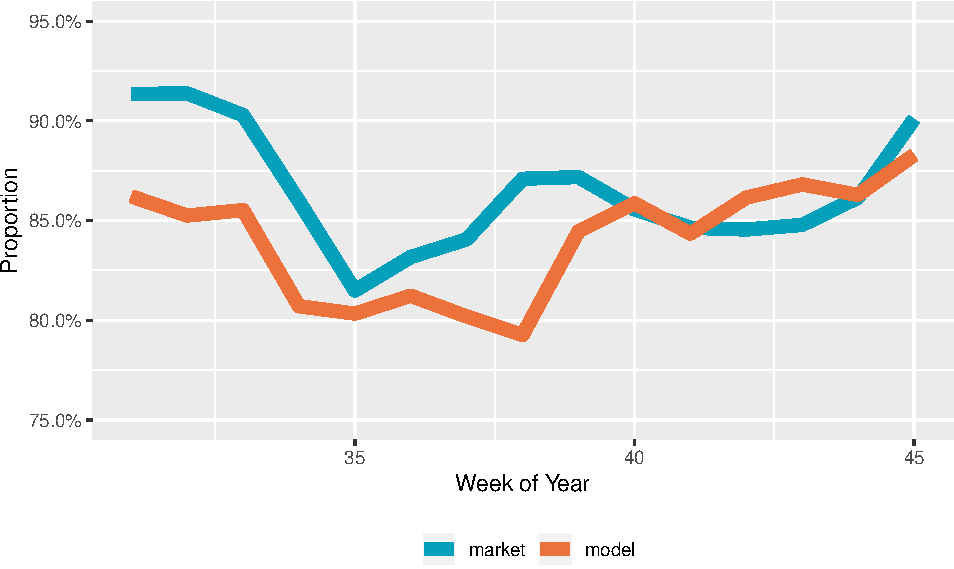
\includegraphics{paper_files/figure-latex/plot_prop_week-1.pdf}
\caption{Proportion of Correct Predictions by Week}
\end{figure}

\begin{figure}
\centering
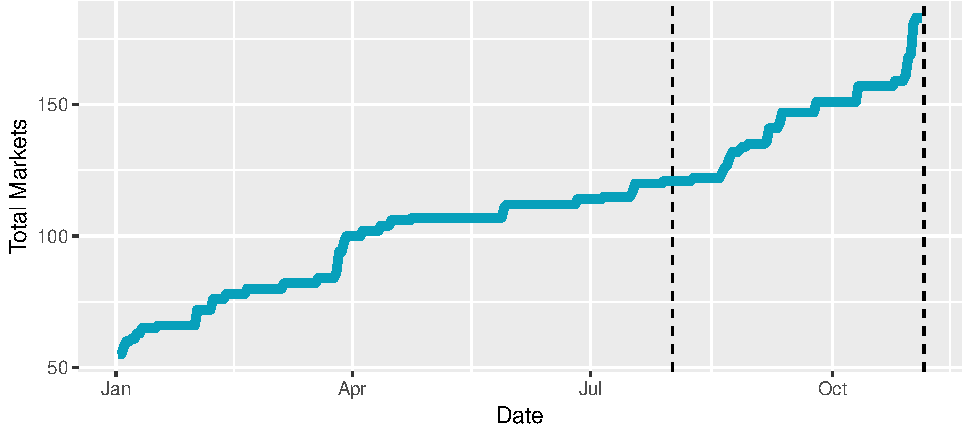
\includegraphics{paper_files/figure-latex/plot_cum_markets-1.pdf}
\caption{Total Number of Election Markets Over Year}
\end{figure}

\begin{figure}
\centering
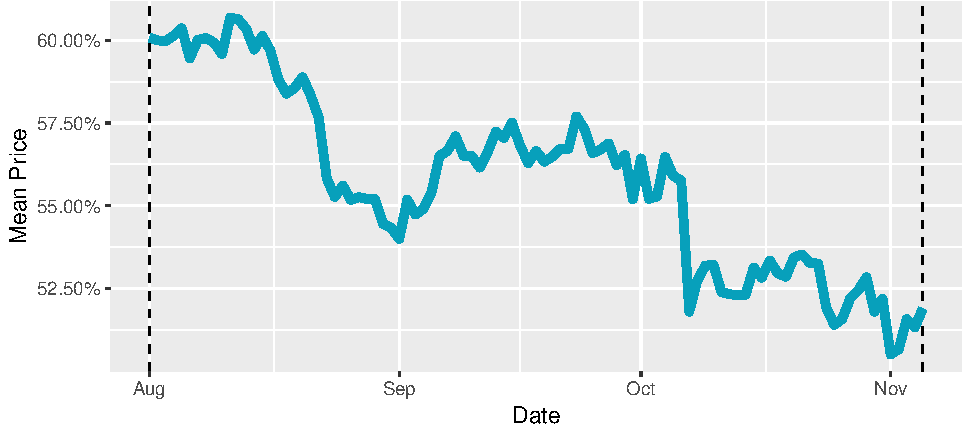
\includegraphics{paper_files/figure-latex/plot_mean_price-1.pdf}
\caption{Mean Democratic Price Over Election}
\end{figure}

This type of binary hit or miss proportion test may not be the ideal
statistical comparison of predictive capabilities. These proportions
tell us how likely any given daily prediction is to being right, but
they do not evaluate how far those predictions are from the truth. This
reductive analysis all but eliminates the probabilistic nature of these
two predictive methods. A prediction giving a candidate a 55\% chance is
treated as accurate and useful as another which gives that same
candidate a 95\% chance. The probabilistic nature of both prediction
markets and forecasting models is what makes them extremely useful tools
for election analysis. It is only at the extreme margins where elections
cross that 50\% threshold. Is there really much value in a candidate's
odds shifting from 51\% one day to 49\% the next? In the test of equal
proportion, these two predictions are treated as entirely opposite
despite very little actually changing in the underlying scenario. In the
115 race sample for the 2018 midterms, a couple elections crossing this
50\% threshold day to day can cause significant changes in the
proportion of ``correct'' predictions. There are better ways to test the
skill of probabilistic forecasts. Looking back at figure 2, You can see
how few of the races are predicted differently. As one would expect, the
unique predictions are all closer to 50\%. It's easy to imagine how a
few of these elections drifting across the 50\% line would affect the
proportion.

\hypertarget{calibration}{%
\subsection{Calibration}\label{calibration}}

One way to further test the predictions is to test them against their
expected accuracy. Inherent in probabilistic predictions is an expected
rate of incorrect predictions. Among all predictions around 70\%, you
would expect only 70\% of those predictions to be correct. From the
graph below (Figure 6), we can see how well each predictive method is
calibrated. Well-calibrated forecasts are as accurate as you'd expect
them to be. Note that the prediction markets are consistently under
confident in Democratic chances when they expect the Democrat to win. Of
races where the Markets predicted the Democrat to have a roughly 60\%
chance of winning, the Democrat ended up winning those elections 85\% of
the time. This nuance is lost in the test for equal proportion.

\begin{figure}
\centering
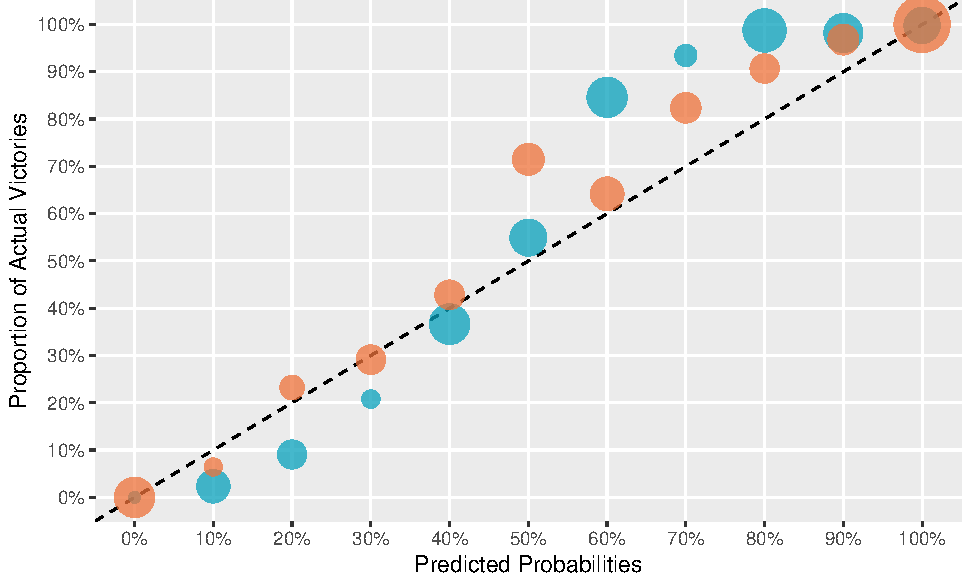
\includegraphics{paper_files/figure-latex/plot_calibration-1.pdf}
\caption{Prediction Calibration}
\end{figure}

\hypertarget{verification}{%
\subsection{Verification}\label{verification}}

The Brier score is allows us evaluate the accuracy of nuanced
probabilistic forecasts tied to mutually exclusive discrete
possibilities. Proposed by Glen Brier in 1950, this function measures
the mean square difference between a probability and the binary outcome.
The function is most often associated with weather forecasting, where
probabilistic forecasts are often assessed on their binary accuracy
(Ferro 2007). In a probabilistic forecast, the error is understood to be
the gap between the probability and the outcome. A correct prediction at
60\% has inherently greater error than the same prediction at 90\%. The
inverse is true for an incorrect prediction. The Brier score evaluates
these errors by summing the squared the difference between forecast and
outcome.

\[
BS={\frac {1}{N}}\sum \limits _{t=1}^{N}(f_{t}-o_{t})^{2}
\]

In the context of these data sets the daily probability (0 to 1) is
subtracted from the outcome (1 for win or 0 for loss). Better
predictions will thus have a lower brier score. A near perfect
prediction will have a brier score of \((0.99-1)^2 = 0.0001\), the worst
predictions would have a brier score of \((0.01-1)^2 = 0.9801\), and a
coin flip prediction would have a score of \((0.50 - 1)^2 = 0.25\)
regardless of outcome. This test allows us to better evaluate the skill
inherent in prediction markets and the forecasting model.

\begin{figure}
\centering
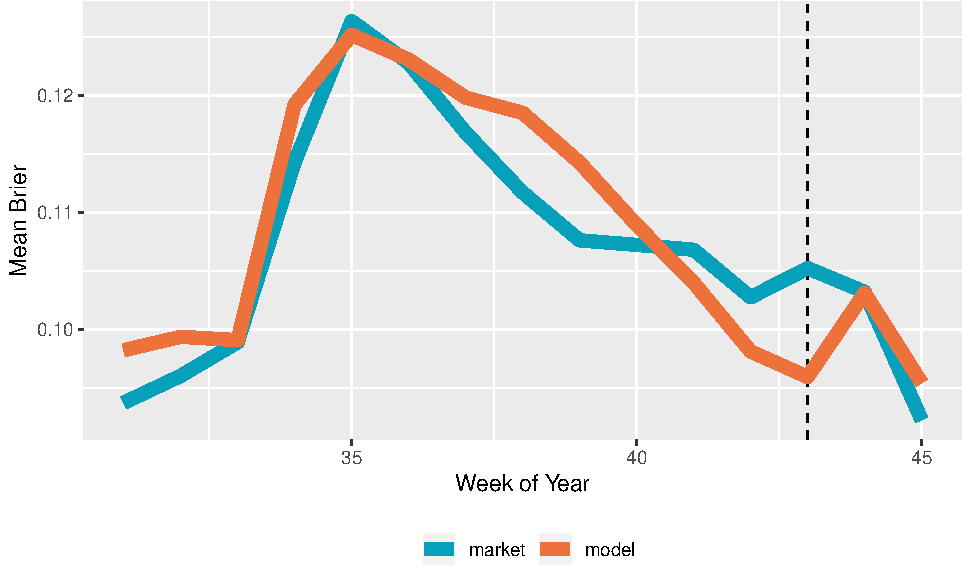
\includegraphics{paper_files/figure-latex/plot_brier_week-1.pdf}
\caption{Mean Brier Scores by Week}
\end{figure}

\begin{longtable}[]{@{}cccc@{}}
\caption{Welch Two Sample t-test: \texttt{brier\_score} by
\texttt{method} (continued below)}\tabularnewline
\toprule
\begin{minipage}[b]{0.21\columnwidth}\centering
Test statistic\strut
\end{minipage} & \begin{minipage}[b]{0.10\columnwidth}\centering
df\strut
\end{minipage} & \begin{minipage}[b]{0.12\columnwidth}\centering
P value\strut
\end{minipage} & \begin{minipage}[b]{0.31\columnwidth}\centering
Alternative hypothesis\strut
\end{minipage}\tabularnewline
\midrule
\endfirsthead
\toprule
\begin{minipage}[b]{0.21\columnwidth}\centering
Test statistic\strut
\end{minipage} & \begin{minipage}[b]{0.10\columnwidth}\centering
df\strut
\end{minipage} & \begin{minipage}[b]{0.12\columnwidth}\centering
P value\strut
\end{minipage} & \begin{minipage}[b]{0.31\columnwidth}\centering
Alternative hypothesis\strut
\end{minipage}\tabularnewline
\midrule
\endhead
\begin{minipage}[t]{0.21\columnwidth}\centering
-0.339\strut
\end{minipage} & \begin{minipage}[t]{0.10\columnwidth}\centering
16943\strut
\end{minipage} & \begin{minipage}[t]{0.12\columnwidth}\centering
0.7346\strut
\end{minipage} & \begin{minipage}[t]{0.31\columnwidth}\centering
two.sided\strut
\end{minipage}\tabularnewline
\bottomrule
\end{longtable}

\begin{longtable}[]{@{}cc@{}}
\toprule
\begin{minipage}[b]{0.30\columnwidth}\centering
mean in group market\strut
\end{minipage} & \begin{minipage}[b]{0.30\columnwidth}\centering
mean in group model\strut
\end{minipage}\tabularnewline
\midrule
\endhead
\begin{minipage}[t]{0.30\columnwidth}\centering
0.1084\strut
\end{minipage} & \begin{minipage}[t]{0.30\columnwidth}\centering
0.1091\strut
\end{minipage}\tabularnewline
\bottomrule
\end{longtable}

Since the Brier score evaluates a historical prediction by summing the
individual prediction scores, a paired t-test can be used to test the
null hypothesis that prediction markets and forecasting models will have
the same mean Brier score (Table 5). When we run such a test, the
statistical significance of the test for equal proportion is put into
question. The mean brier score for all market predictions is 0.1084,
compared to 0.1091 for the model. With a p-value of 0.7346, there is no
way to claim a statistically significant difference in these two scores
across the history of the election. Only during the week of October 22nd
was there a statistically significant difference in the mean Brier
scores for each method, with the model slightly outperforming the market
\((model = 0.105, market = 0.959, p = 0.0008)\). By using Brier scores
instead of reductive proportions, we can now see that any difference in
these two predictive methods is actually minimal and unhelpfully
accentuated by using the 50\% delineator to test right from wrong.

\hypertarget{conclusion}{%
\section{Conclusion}\label{conclusion}}

Both predictive methods are fairly well calibrated and can predict
elections with a useful degree of accuracy. Considering the sample of
races compared and analyzed contains the most contentious races, the
upwards of 80\% accuracy is impressive. While the predictions markets
were able to predict significantly more of the sample races correctly,
especially earlier in the election, the actual skill difference between
these two methods is negligible. This difference stems from the
confidence in each method. From the table below, you can see the mean
probabilities for correct and incorrect predictions. For races where the
Democrat was predicted to win and did win, the forecasting model was 5\%
more confident. For races where the Democrat was correctly predicted to
lose, the model is over 6\% more confident (Table 6). This disparity may
stem from the demographic bias of the traders; \emph{PredictIt} has
acknowledged that the vast majority of traders are young, white,
conservative men. While they appear to be more capable at predicting the
overall winner of the election, the traders seem to demonstrate a bias
against Democratic candidates. The traders demonstrate a similar
underestimation of incumbent candidates, giving incumbent Democrats over
10\% lower odds compared to the forecasting model (Table 7). These
potential biases should be kept in mind when using prediction markets as
a tool. The trading volume should also be kept in mind and more research
needs to be done into the effect volume has on predictive accuracy.

\begin{longtable}[]{@{}llrr@{}}
\caption{Mean Probabilities by Prediction and Outcome}\tabularnewline
\toprule
Prediction & Election & Market & Model\tabularnewline
\midrule
\endfirsthead
\toprule
Prediction & Election & Market & Model\tabularnewline
\midrule
\endhead
FALSE & FALSE & 0.230 & 0.168\tabularnewline
FALSE & TRUE & 0.406 & 0.365\tabularnewline
TRUE & FALSE & 0.593 & 0.637\tabularnewline
TRUE & TRUE & 0.795 & 0.845\tabularnewline
\bottomrule
\end{longtable}

\begin{longtable}[]{@{}lrr@{}}
\caption{Mean Probabilities by Incumbency}\tabularnewline
\toprule
Incumbent & Market & Model\tabularnewline
\midrule
\endfirsthead
\toprule
Incumbent & Market & Model\tabularnewline
\midrule
\endhead
FALSE & 0.487 & 0.471\tabularnewline
TRUE & 0.793 & 0.905\tabularnewline
\bottomrule
\end{longtable}

\hypertarget{bibliography}{%
\section*{Bibliography}\label{bibliography}}
\addcontentsline{toc}{section}{Bibliography}

\hypertarget{refs}{}
\leavevmode\hypertarget{ref-arrow08promise}{}%
Arrow, Kenneth J., Robert Forsythe, Michael Gorham, Robert Hahn, Robin
Hanson, John O. Ledyard, Saul Levmore, et al. 2008. ``The Promise of
Prediction Markets.'' \emph{Science} 320 (5878): 877--78.
\url{http://www.jstor.org/stable/20054723}.

\leavevmode\hypertarget{ref-berg14iem}{}%
Berg, Joyce E., and Thomas A. Rietz. 2014. ``Market Design,
Manipulation, and Accuracy in Political Prediction Markets: Lessons from
the Iowa Electronic Markets.'' \emph{PS: Political Science and Politics}
47 (2): 293--96. \url{http://www.jstor.org/stable/43284536}.

\leavevmode\hypertarget{ref-fair09uncertainty}{}%
Fair, Ray C. 2009. ``Interpreting the Predictive Uncertainty of
Elections.'' \emph{The Journal of Politics} 71 (2): 612--26.
\url{http://www.jstor.org/stable/10.1017/s0022381609090495}.

\leavevmode\hypertarget{ref-ferro07brier}{}%
Ferro, Christopher A. T. 2007. ``Comparing Probabilistic Forecasting
Systems with the Brier Score.'' \emph{Weather and Forecasting} 22 (5):
1076--88. \url{https://doi.org/10.1175/WAF1034.1}.

\leavevmode\hypertarget{ref-grim16wrong}{}%
Grim, Ryan. 2016. ``Nate Silver Is Unskewing Polls -- All Of Them -- In
Trump's Direction.'' \emph{HuffPost}, November.
\url{https://www.huffpost.com/entry/nate-silver-election-forecast_n_581e1c33e4b0d9ce6fbc6f7f}.

\leavevmode\hypertarget{ref-lubridate}{}%
Grolemund, Garrett, and Hadley Wickham. 2011. ``Dates and Times Made
Easy with lubridate.'' \emph{Journal of Statistical Software} 40 (3):
1--25. \url{http://www.jstatsoft.org/v40/i03/}.

\leavevmode\hypertarget{ref-oliven04suckers}{}%
Oliven, Kenneth, and Thomas A. Rietz. 2004. ``Suckers Are Born but
Markets Are Made: Individual Rationality, Arbitrage, and Market
Efficiency on an Electronic Futures Market.'' \emph{Management Science}
50 (3): 336--51. \url{http://www.jstor.org/stable/30046071}.

\leavevmode\hypertarget{ref-base}{}%
R Core Team. 2018. \emph{R: A Language and Environment for Statistical
Computing}. Vienna, Austria: R Foundation for Statistical Computing.
\url{https://www.R-project.org/}.

\leavevmode\hypertarget{ref-verification}{}%
Research Applications Laboratory, NCAR -. 2015. \emph{Verification:
Weather Forecast Verification Utilities}.
\url{https://CRAN.R-project.org/package=verification}.

\leavevmode\hypertarget{ref-rhode06manip}{}%
Rhode, Paul, and Koleman Strumpf. 2006. ``Manipulating political stock
markets: A field experiment and a century of observational data.''
Natural Field Experiments 00325. The Field Experiments Website.
\url{https://ideas.repec.org/p/feb/natura/00325.html}.

\leavevmode\hypertarget{ref-wayback}{}%
Rudis, Bob. 2017. \emph{Wayback: Tools to Work with Internet Archive
Wayback Machine Apis}. \url{https://github.com/hrbrmstr/wayback}.

\leavevmode\hypertarget{ref-ggplot2}{}%
Wickham, Hadley. 2016. \emph{Ggplot2: Elegant Graphics for Data
Analysis}. Springer-Verlag New York.
\url{https://ggplot2.tidyverse.org}.

\leavevmode\hypertarget{ref-stringr}{}%
---------. 2019. \emph{Stringr: Simple, Consistent Wrappers for Common
String Operations}. \url{https://CRAN.R-project.org/package=stringr}.

\leavevmode\hypertarget{ref-dplyr}{}%
Wickham, Hadley, Romain François, Lionel Henry, and Kirill Müller. 2019.
\emph{Dplyr: A Grammar of Data Manipulation}.
\url{https://CRAN.R-project.org/package=dplyr}.

\leavevmode\hypertarget{ref-tidyr}{}%
Wickham, Hadley, and Lionel Henry. 2019. \emph{Tidyr: Easily Tidy Data
with 'Spread()' and 'Gather()' Functions}.
\url{https://CRAN.R-project.org/package=tidyr}.

\leavevmode\hypertarget{ref-readr}{}%
Wickham, Hadley, Jim Hester, and Romain Francois. 2018. \emph{Readr:
Read Rectangular Text Data}.
\url{https://CRAN.R-project.org/package=readr}.




\newpage
\singlespacing 
\end{document}
